%!TEX root = ../draft.tex
\chapter{Methodik und Durchführung}\label{s.methudurchf}
In diesem Kapitel werden die verwendeten Datensätze aufgeführt und die Umsetzung der Normalisierungsalgorithmen beschrieben.  
 \section{Vortrainierte Netze}\label{s.modell}
Das Unternehmen COCO \cite{common2018data} (Common Objects in Contexts) stellt eine Vielzahl an Datensätzen bereit, mit denen neuronale Netze trainiert werden können. Bei den Datensätzen handelt es sich um unterschiedliche Objekte in verschiedenen Umgebungen.  
Einige Netze, welche mit den COCO-Datensätzen trainiert wurden, stehen als \textit{Open Source} zur Verfügung. Die folgende Tabelle \ref{tab:cocomodels} führt ausgewählte neuronale Netze auf, um Genauigkeit und Geschwindigkeit vergleichen zu können, damit ein geeignetes Netz für die Versuche ausgewählt werden kann.
\begin{table}
[h]
\caption{Künstliche neuronale Netze \cite{google2018tens}, welche mit dem COCO Dataset trainiert wurden \cite{common2018data}} 
\label{tab:cocomodels}
\centering
\begin{tabular}{|l|c|c|}
\hline
Neuronales Netz & mAP & Geschwindigkeit\\
\hline
faster\_rcnn\_inception\_v2\_coco & 28 & 58\\
faster\_rcnn\_resnet50\_coco & 30 & 89\\
rfcn\_resnet101\_coco & 30 & 92\\
ssd\_mobilenet\_v1\_coco & 30 & 21\\
ssd\_resnet\_50\_fpn\_coco & 35 & 76\\
\hline
\end{tabular}
\end{table}
Um die Auswirkungen der Normalisierung deutlich hervorheben zu können, wurde ein Netz ausgewählt, welches eine recht niedrige mAP hat. Deswegen wurde das faster\_rcnn\_inception\_v2\_coco ausgewählt. Es hat eine \textit{mAP} von 28 und eine Geschwindigkeit von 32 ms. Dadurch, dass es die niedrigste \textit{mAP} hat, sollten die Auswirkungen der Normalisierungsverfahren genauer erkennbar sein, als bei Netzen mit einer höheren mAP. Das ausgewählte Netz wird im Folgenden auf die Datensätze, welche im anschließenden Unterkapitel aufgeführt sind, angewendet.
  \section{Trainingsdaten}\label{s.tdaten}
Wie bereits in Kapitel \ref{s.trainingsdaten} beschrieben, werden zum trainieren eines neuronalen Netzes üblicherweise mehrere hunderttaused Daten benötigt. Durch die Verwendung eines vortrainierten Netzes, werden für das Trainieren der eigenen Klassen nur noch durchschnittlich 150 Bilder pro Objektklasse benötigt. Das hat eine deutliche Verkürzung der Trainingsdauer zur Folge. Die Bilder der eigenen Daten werden mit einer 13-Megapixel-Kamera eines \textit{Huawei P Smart} aufgenommen. Die verwendeten Objekte werden von vielen verschiedenen Seiten aufgenommen. Da die erstellten Bilder mehrere Megabyte groß sind, müssen diese auf 100-300 KB komprimiert werden. Wie auch der Test später zeigen wird, verlängern sich die Laufzeiten der Algorithmen exponentiell, je größer das Bild ist.\\
Damit am Ende des Projektes möglichst gute Vergleichswerte entstehen, werden mehrere Datensätze für den Versuch verwendet. Insgesamt werden die neuronalen Netze mit drei unterschiedlichen Datensätzen trainiert. Der erste Datensatz, welcher getestet wird, ist der Nahrungsmittel-Datensatz eines früheren Projektes, der Zweite der Datensatz von \textit{Pascal Visual Object Classes} (PascalVOC) und der Dritte der Hunderassen-Datensatz, Stanford Dog Dataset.\\
In den folgenden Tabellen werden alle Datensätze mit den dazugehörigen Klassen aufgeführt:\\\\
Der erste Datensatz besteht aus sechs Klassen, welche in der Tabelle \ref{tab:nahrungsmittel} aufgeführt sind. Jede Klasse besitzt um die 100-150 Bilder, die zusätzlich Annotations-Dateien mit den Koordinaten der Klassifizierungsboxen (Kapitel \ref{s.trainingsdaten}) beinhalten. Dieser Datensatz ist mit seinen ca. 1.000 Bildern der kleinste Datensatz. 
\begin{table}
[h]
\caption{Datensatz mit Nahrungsmitteln}
\centering
\begin{tabular}{|l|l|}
\hline
Klassenname & Klassenname\\
\hline
Milch - Packung & Orangensaft - Packung\\
Wasser - Flasche & Bier - Flasche\\
Brunch - Aufstrich & Margarine - Aufstrich\\
\hline
\end{tabular}
\label{tab:nahrungsmittel}
\end{table}
Der PascalVOC-Datensatz umfasst 20 Klassen und besteht aus 5.000 Bildern. Von 2005 bis 2012 wurde jährlich die PascalVOC-Challenge durchgeführt. Dabei sollte das beste Verfahren für die Segmentierung, Klassifikation und Objekterkennung ermittelt werden. Inhaltlich befasst sich der Datensatz mit einer Reihe unterschiedlicher Klassen, welche in Tabelle \ref{tab:pvoc} zu erkennen sind. Es gibt einige Unterschiede in der Häufigkeit der auftretenden Klassen. Beispielsweise sind in rund 2.000 Bildern insgesamt 4.690 Personen enthalten, weswegen es möglicherweise Unterschiede in der Genauigkeit der Klassen geben könnte. Die Aufnahmen der Bilder sind thematisch und von der Art der Aufnahme unstrukturiert, was bedeutet, dass teilweise Bilder von einzelnen Objekten, Gruppen von Objekten oder auch ganze Szenen enthalten sind.
\begin{table}
[h]
\caption{Pascal Visual Object Classes \cite{pascal-voc-2007}}
\centering
\begin{tabular}{|l|l|l|l|}
\hline
Klassenname & Klassenname & Klassenname & Klassenname\\
\hline
Person & Vogel & Katze & Kuh\\
Hund & Pferd & Schaf & Zug\\
Flugzeug & Fahrrad & Boot & Bus\\
Auto & Motorrad & Flasche & Stuhl\\
Tisch & Blumentopf & Sofa & Bildschirm\\
\hline
\end{tabular}
\label{tab:pvoc}
\end{table}
Der dritte Datensatz, welcher in dieser Arbeit verwendet wird, ist der Hunde-Datensatz aus Stanford und beinhaltet 120 verschiedene Hunderassen. Jede Klasse hat um die 200 Bilddaten. Wegen der Struktur des Datensatzes, in einzelnen Ordnern, kann eine Auswahl der priorisierten Hunderassen zusammengestellt werden. Für den Versuch und damit eine bessere Übersicht erreicht werden kann, wurden 20 Hunderassen ausgewählt. Die Anotationen der Daten sind in Form von XML-Dateien beigefügt. In der Tabelle \ref{tab:sdd} werden die ausgewählten Klassen des Datensatzes zusammengefasst.
\begin{table}
[h]
\caption{Stanford Dog Dataset \cite{KhoslaYaoJayadevaprakashFeiFei_FGVC2011}}
\label{tab:sdd}
\centering
\begin{tabular}{|l|l|l|l|}
\hline
Klassenname & Klassenname & Klassenname & Klassenname\\
\hline
Chihuahua & Japanese Spaniel & Maltese Dog & Pekinese\\
Shih-Tzu & Blenheim Spaniel & Papillon & Toy Terrier\\
Rhodesian Ridgeback & Afghan Hound & Basset & Beagle\\
Bloodhound & Bluetick & Coonhound & Walker Hound\\
Redbone & Borzoi & Irish Wolfhound & Italian Greyhound\\
\hline
\end{tabular}
\end{table}
Die Struktur der Datensätze ist ähnlich aufgebaut. Das heißt, viele verschiedene Klassen mit verschiedenen Szenen und Kontexten. Im Folgenden wird zunächst auf die Umsetzung der Normalisierungsverfahren eingegangen, um weitere Erkenntnisse zu erlangen.
\section{Normalisierungs-Algorithmen}\label{s.nalgorithmen}
Für die Normalisierung der Datensätze ist eine Methode nötig, mit der mehrere Bilder möglichst schnell hintereinander bearbeitet werden können. Für die Normalisierung wurden Python-Programme geschrieben, welche nacheinander die Bilder, anhand eines Algorithmus, verarbeiten. Dafür wurden mitunter die \textit{Python Image Libary} und OpenCV genutzt. Beide Bibliotheken werden für das Verarbeiten von Bildern benötigt. 
\newpage
\subsection{Gray-World-Algorithmus} 
Im Folgenden wird der Codeblock für den Gray-World-Algorithmus aufgeführt, wie er in den Versuchen verwendet wurde.\\
\begin{lstlisting}
image = cv.imread(i, 1)
image = image.transpose(2, 0, 1).astype(np.uint32)
averageGreenChannel = np.average(image[1])
image[0] = np.minimum(image[0]*(avgGreen/np.average(image[0])),255)
image[2] = np.minimum(image[2]*(avgGreen/np.average(image[2])),255)
img_output = image.transpose(1, 2, 0).astype(np.uint8)
\end{lstlisting}
???Der Gray-World-Algorithmus \cite{gray2012world}, welcher hier verwendet wird, funktioniert etwas anders, als in den Grundlagen beschrieben. Für die Normalisierung der Kanäle wird der Durchschnitt des Grünkanals verwendet, da diese Farbe wichtig für das Helligkeitsempfinden ist. Zunächst wird in Zeile 1, das zu normalisierende Bild mittels OpenCV importiert. In der Zeile 2 wird der Farbraum des Bildes in 32 Bit umgewandelt. Daraufhin wird in Zeile 6 der Durchschnittswert des Grünkanals berechnet und zwischengespeichert. In der Zeile 8 wird der Grünkanal nun mit dem Durchschnitt des Rotkanals dividiert und anschließend mit dem Minimum des Rotkanals multipliziert und übernommen. Der gleiche Vorgang erfolgt mit dem Blaukanal in Zeile 10. Abschließend wird das bearbeitete Bild in 8 Bit umgewandelt und ausgegeben (Abbildung \ref{img:gwnimg}). 
\begin{figure}
	[h]
	\centering
	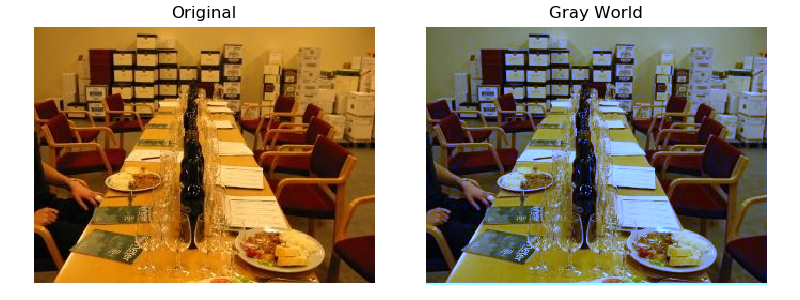
\includegraphics[scale=0.6]{Sources/gwn.png}
	\caption{Auswirkung des Gray-World-Algorithmus}
	\label{img:gwnimg}
\end{figure}
\newpage
\subsubsection{Histogramm-Ausgleich}
Weiter geht es mit dem ersten Histogramm-Normalisierungsverfahren, der Histogramm-Ausgleichung. Diese wird im Folgenden aufgeführt und beschrieben.\\
\begin{lstlisting}
image = cv.imread('input.jpg')
image_yuv = cv.cvtColor(image, cv.COLOR_BGR2YUV)
image_yuv[:,:,0] = cv.equalizeHist(image_yuv[:,:,0])
img_output = cv.cvtColor(image_yuv, cv.COLOR_YUV2BGR)
\end{lstlisting}
Für die Histogramm-Ausgleichung \cite{histogram2012equalisation} wird das Bild in Zeile 3 vom BGR-Farbraum in den YUV-Farbraum (Unterabschnitt \ref{s.lab} umgewandelt. Der Y-Kanal wird für die Histogramm-Ausgleichung verwendet. Das hat den Grund, dass das Luminanzsignal oder auch Leuchtdichte-Signal die Summe der drei Grundfarben Rot Grün und Blau und die Helligkeitsinformation enthält. In Zeile 4 wird das Histogramm des Y-Kanals, wie in Abschnitt \ref{s.histogramme} beschrieben, ausgeglichen. Das normalisierte Bild wird von dem YUV-Farbraum zurück in den BGR-Farbraum konvertiert und zwischengespeichert. Das Ergebnis wird als Bild ausgegeben (Abbildung \ref{img:histogrameq}).
\begin{figure}
	[h]
	\centering
	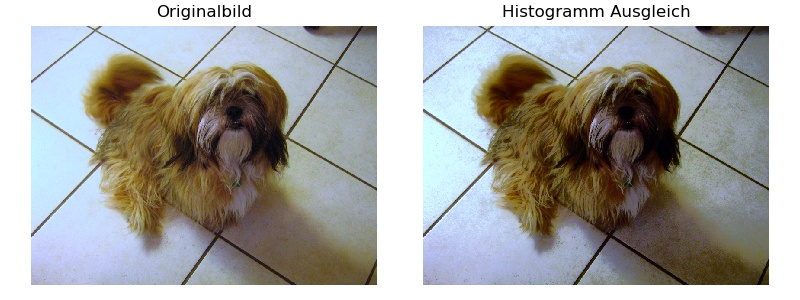
\includegraphics[scale=0.7]{Sources/histeq.jpg}
	\caption{Auswirkung der Histogramm-Ausgleichung}
	\label{img:histogrameq}
\end{figure}	
\newpage
\subsection{Histogramm-Spezifikation}
Der letzte Algorithmus, welcher geprüft wird, ist die Histogramm-Spezifikation. Hier wird kurz auf die Umsetzung und ein Beispielergebnis eingegangen.\\
\begin{lstlisting}
reference_image = io.imread('reference_image.jpg')
source_image = io.imread('source_image.jpg')
matched_image = match_histograms(source_image, reference_image, multichannel=True)
\end{lstlisting}
Die dritte Normalisierungsfunktion, die auf die Datensätze angewendet wird, ist die Histogramm-Spezifikation (Unterabschnitt \ref{s.hs}) oder auch \textit{Histogramm Matching}. Für den Algorithmus wird die Python-Bibliothek \textit{Scikit-image} verwendet. Hierfür werden ein Referenzbild und ein Zielbild geladen. Diese beiden Bilder werden mit der Funktion \textit{match\_histograms} verarbeitet. Das Zielbild wurde auf das Histogramm des Referenzbildes angepasst. In dem Beispiel \ref{img:histogramspez} kann man gut erkennen, dass das Quellbild, welches stark verdunkelt ist, durch ein gut ausgeleuchtetes Referenzbild, eine wesentlich bessere Helligkeit aufweist. Die Problematik bei dieser Normalisierungs-Methode besteht darin, dass ein einheitliches Referenzbild genutzt werden muss, auf welchem dann der gesamte Datensatz normalisiert wird.
\begin{figure}
	[h]
	\centering
	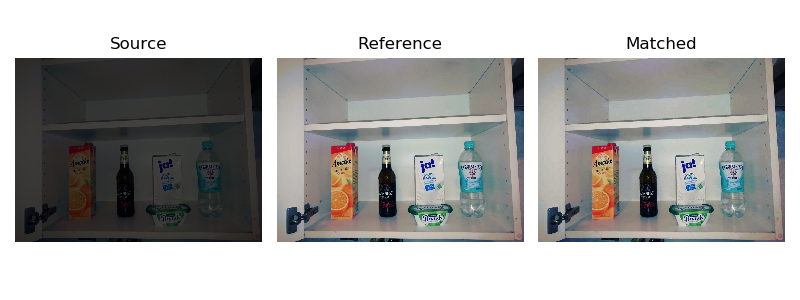
\includegraphics[scale=0.6]{Sources/HS_beispiel.png}
	\caption{Das Zielbild wurde mithilfe des Referenzbildes ausgeglichen und angepasst. Auf der linken Seite ist das Ergebnis der Spezifikation.}
	\label{img:histogramspez}
\end{figure}